\documentclass{letask}

\begin{document}
\begin{titlepage}
\center % Center everything on the page
 
%----------------------------------------------------------------------------------------
%	HEADING SECTIONS
%----------------------------------------------------------------------------------------

\textsc{\LARGE Московский\\[-0.2cm]Физико-Технический Институт\\[0.1cm]\large (государственный университет)}\\[1.5cm] % Name of your university/college
\textsc{\Large Кафедра общей физики}\\[0.1cm] % Major heading such as course name
\textsc{\large Лабораторная работа \textnumero  4.4.1}\\[0.5cm] % Minor heading such as course title

%----------------------------------------------------------------------------------------
%	TITLE SECTION
%----------------------------------------------------------------------------------------

\HRule
\\[0.4cm]
{ \huge \bfseries Амплитудная\\[0.2cm]
дифракционная решетка}
\\[0.6cm] % Title of your document
\HRule
\\[1.5cm]


 
%----------------------------------------------------------------------------------------
%	AUTHOR SECTION
%----------------------------------------------------------------------------------------

\begin{minipage}{0.4\textwidth}
	\begin{flushleft} \large
		\textsf{Студент}
		
		Ришат \textsc{Исхаков} \\[-0.15cm]
		513 группа
	\end{flushleft}
\end{minipage}
~
\begin{minipage}{0.4\textwidth}
	\begin{flushright} \large
		\textsf{Преподаватель}
		
		Александр Александрович \\[-0.15cm]
		\textsc{Казимиров} % Supervisor's Name
	\end{flushright}
\end{minipage}

\begin{bottompar}
	\begin{center}
		
\includegraphics[width = 80 mm]{logo.jpg}
	\end{center}
	{\large \today}

\end{bottompar}
\vfill % Fill the rest of the page with whitespace

\end{titlepage}

\textbf{Цель работы:} Ознакомление с методами получения и анализа поляризованного света.

\textbf{В работе используются:} Оптическая скамья с осветителем, зеленый светофильтр, два поляроида, черное зеркало, полированная эбонитовая пластинка, стопа стеклянных пластинок, слюдяные пластинки разной толщины, пластинки в 1/4 и 1/2 длины волны, пластика в одну длины волны для зеленого цвета (пластинка чувствительного оттенка).
 
\section{Теоретическая часть}

\subsection{Определение направления разрешенной плоскости колебаний поляроида}

Определить направление разрешённых колебаний поляроида проще всего с помощью чёрного зеркала.

Вращая поляроид вокруг направления луча и чёрное зеркало вокруг
оси, перпендикулярной лучу, методом последовательных приближений
можно добиться минимальной яркости луча, отражённого от зеркала,
и таким образом определить разрешённое направление поляроида.


\subsection{Получение эллиптически поляризованного света}

Эллиптически
поляризованный свет можно получить из линейно поляризованного с
помощью двоякопреломляющих кристаллических пластинок.

Двоякопреломляющая пластинка имеет два взаимно перпендикулярных главных направления, совпадающих с осями эллипсоида диэлектрической проницаемости. Волны, поляризованные вдоль главных направлений, распространяются в пластинке с разными скоростями, не изменяя характера своей поляризации. Эти волны называются главными. 

Сдвиг фаз при проходе через такую пластинку определяется соотношением:

\[\Delta \varphi = \dfrac{2\pi}{m} = kd(n_x-n_y)\]

Рассмотрим три частных случая:
\begin{itemize}
\item Пластинка дает сдвиг фаз на $2\pi$ (пластинка в длину волны $\lambda$). Тогда на выходе будет линейно поляризованная волна с тем же направлением колебаний, что и в падающей волне.
\item Пластинка дает сдвиг фаз $\pi$ (пластинка в пол длины волны $\lambda/2$). На выходе образуется линейно поляризованная волна с направлением колебаний, зеркально отраженным относительно одного из главных направлений.
\item Пластинка создает между колебаниями сдвиг фаз $\pi/2$ (пластинка в четверть длины волны $\lambda/4$). Образуется эллипс, главные оси которого совпадают с координатными осями x и y.
\end{itemize}

\subsection{Анализ эллиптически поляризованного света}


Анализ эллиптически поляризованного света сводится к нахождению главных осей
эллипса поляризации и к определению направления вращения электрического вектора.

Главные оси эллипса поляризации определяются с помощью анализатора по максимуму и минимуму интенсивности проходящего света.
Направление вращения электрического вектора может быть найдено с помощью пластинки в четверть длины волны, для которой известно,
какая из главных волн, $E_x$ или $E_y$ , имеет большую скорость распространения (и соответственно меньшее значение показателя преломления).

\subsection{Пластинка чувствительного оттенка}

Так называют пластинку в $\lambda$ для зеленой спектральной компоненты $560~\nm$.

\begin{figure}[H]
\centering
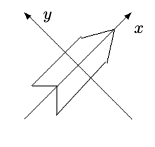
\includegraphics[width=0.2\linewidth]{1}
\caption{Пластинка чувствительного оттенка}
\end{figure}

Если пластинка чувствительного оттенка помещена между скрещенными поляроидами и главные направления пластинки не параллельны
направлениям разрешённых колебаний поляроидов, то при освещении
белым светом пластинка кажется окрашенной в лилово-красный цвет.

Если между скрещенными поляроидами поместить еще пластинку в $\lambda/4$, чтобы их главные направления совпадали, цвет будет казаться зеленовато-голубым.

Если главные направления будут перпендикулярны, то цвет будет оранжево-желтым.


\section{Схема установки}

\begin{figure}[H]
\centering
\begin{minipage}[h]{0.24\linewidth}
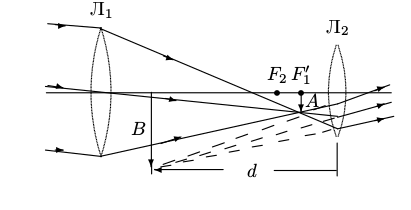
\includegraphics[width=1\linewidth]{2}
\label{1}
\caption{Определение разрешенного направления поляроида} 
\end{minipage}
\hfill 
\begin{minipage}[h]{0.24\linewidth}
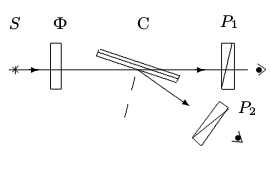
\includegraphics[width=1\linewidth]{3}
\label{2}
\caption{Исследование стопы}
\end{minipage}
\hfill 
\begin{minipage}[h]{0.24\linewidth}
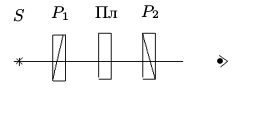
\includegraphics[width=1\linewidth]{4}
\label{3}
\caption{Определение главных направлений в пластинках}
\end{minipage}
\hfill 
\begin{minipage}[h]{0.24\linewidth}
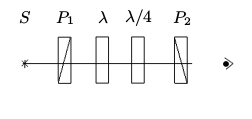
\includegraphics[width=1\linewidth]{5}
\label{4}
\caption{Определение направлений большей и меньшей скорости}
\end{minipage}
\end{figure}

\underline{Характеристики установки:}


\section{План работы}

\begin{enumerate}
\item Определение разрешенных направлений поляроидов

Добиваемся минимальной яркости отраженного от зеркала луча, добавляем второй поляроид и проделываем то же самое.

\item Определение угла Брюстера для эбонита

Заменяем чёрное зеркало эбонитовой пластинкой. Определяем угол Брюстера, откуда находим показатель преломления. Сравниваем интенсивность со светофильтром и без него.

\item Исследование стопы

Подбираем положение стопы, при котором свет падает на неё под углом Брюстера. Определяем характер поляризации: вектор Е в отражённом луче перпендикулярен плоскости преломления, в проходящем – параллелен, как и предполагала теория.

\item Определение главных плоскостей двоякопреломляющих пластин.

При совпадении главных осей пластинки со скрещенными разрешенными направлениями поляроидов интенсивность света минимальная.

\item Выделение пластин $\lambda/2$ и $\lambda/4$ 



\end{enumerate}


\section{Ход работы и обработка результатов}

\begin{enumerate}
\item Определение разрешенных направлений поляроидов 

$\varphi_{\text{пол}1} = 2^\circ \pm 1^\circ$
\hspace{5cm}
$\varphi_{\text{пол}2} = 84^\circ \pm 1^\circ$


\item Определение угла Брюстера для эбонита (Как в предыдущем пункте, но с эбонитом вместо черного зеркала)

$\theta = 58^\circ \pm 2^\circ$

$ n = \tan{\theta} = 1,6 \pm 0,1 $

При добавленном светофильтре $\theta$ не изменилось.

\item Исследование стопы

Отраженный луч поляризован, вектор $E$ перпендикулярен плоскости преломления, преломленный частично поляризован.

\item Определение главных направлений двоякопреломляющих пластин 

Для пластины 1 $min = 52^\circ \pm 1^\circ$ и $max = 0^\circ \pm 1^\circ$

Для пластины 2 $min = 345^\circ \pm 1^\circ$ и $max = 36\circ \pm 1^\circ$

Для пластины 1 проходящий свет имел эллиптическую поляризацию, то есть пластина 1 -- $\lambda/4$. Для пластины 2 линейную, то есть пластина 2 --  $\lambda/2$.

\item Определение быстрой и медленной оси в пластинке $\lambda/4$


При вращении пластинки относительно пластинки чувствительного оттенка цвет стрелки менялся от голубого до желтого. В положении, когда цвет голубой, быстрые направления пластинок совпадают, когда желтый, они перпендикулярны.

\item Исследование интерференции поляризованных лучей.

При вращении мозаичной пластинки изменялась интенсивность, при вращении поляроида менялся цвет пластинок.

\end{enumerate}

\section{Вывод}
Ознакомились с методами получения и анализа поляризованного света, измерили коэффициент преломления эбонита, исследовали двоякопреломляющие пластины.
\end{document}

\section{Установка и измерения}

\section{Вывод}

\end{document}
